\begin{enumerate}
	\item
		\begin{minipage}[t]{\linewidth}
		\raggedright
		Verbindt de gedownloade ISO aan de virtuele CD speler door in het Settings menu op storage te clicken en het bestand te koppelen aan de CD.
		\adjustbox{valign=t}{%
			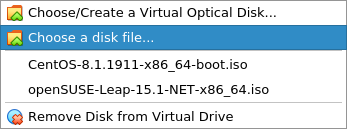
\includegraphics[width=0.99\linewidth]{linuxreader-img006.png}%
		}
		\end{minipage}
	\item Nu mag je de virtuele machine opstarten. Het eerste scherm dat je tegen komt geeft je de mogelijkheid om CentOS te installeren en dat gaan we dan ook doen.
	\item
		\begin{minipage}[t]{\linewidth}
		\raggedright
		Je kan wachten tot de installatie automatisch start of je drukt op enter om de installatie te starten.
		\adjustbox{valign=t}{%
			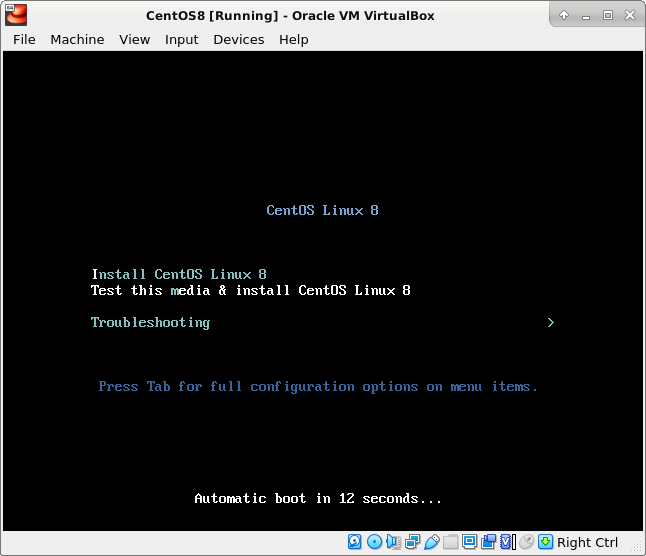
\includegraphics[width=0.99\linewidth]{linuxreader-img007.png}%
		}
		\end{minipage}
	\item
		\begin{minipage}[t]{\linewidth}
		\raggedright
		\adjustbox{valign=t}{%
			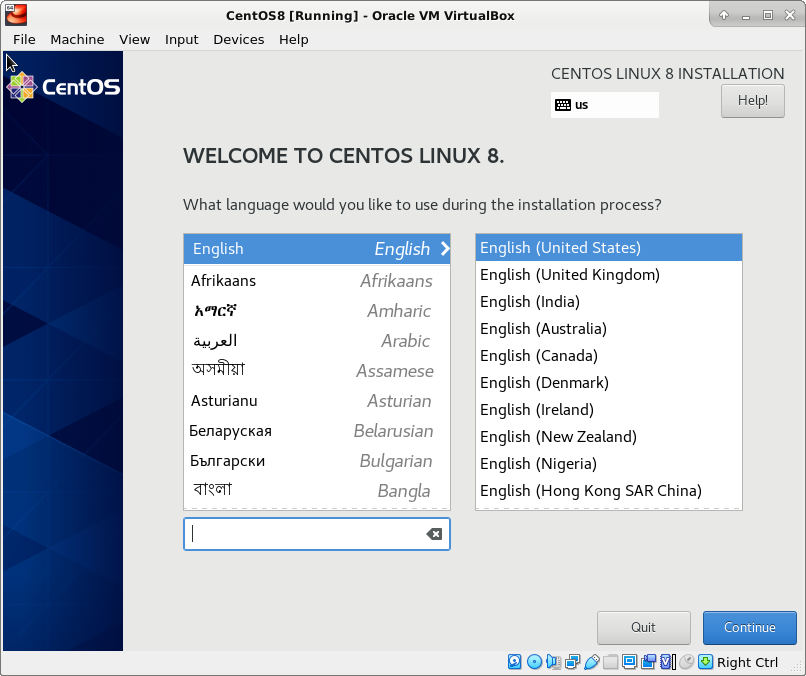
\includegraphics[width=0.99\linewidth]{linuxreader-img008.png}%
		}
		Het is misschien het handigst om een systeem in de Engelse taal te installeren, deze cursus gaat daarvan uit. Het grote voordeel is dat als je iets wil zoeken op het Internet dat je dan al gelijk in het Engels zoekt wat de kans op gelijksoortige problemen groter maakt er zijn immers meer mensen die Engels spreken dan Nederlands. Maar als je je niet vertrouwd genoeg vindt in het Engels dan kan je hier ook kiezen voor een Nederlandstalige installatie.
		\end{minipage}
	\item
		\begin{minipage}[t]{\linewidth}
		\raggedright
		In het vervolg scherm heb je heel veel keuzes in 1 keer. We zullen ze in de meest logische volgorde doorlopen.
		\adjustbox{valign=t}{%
			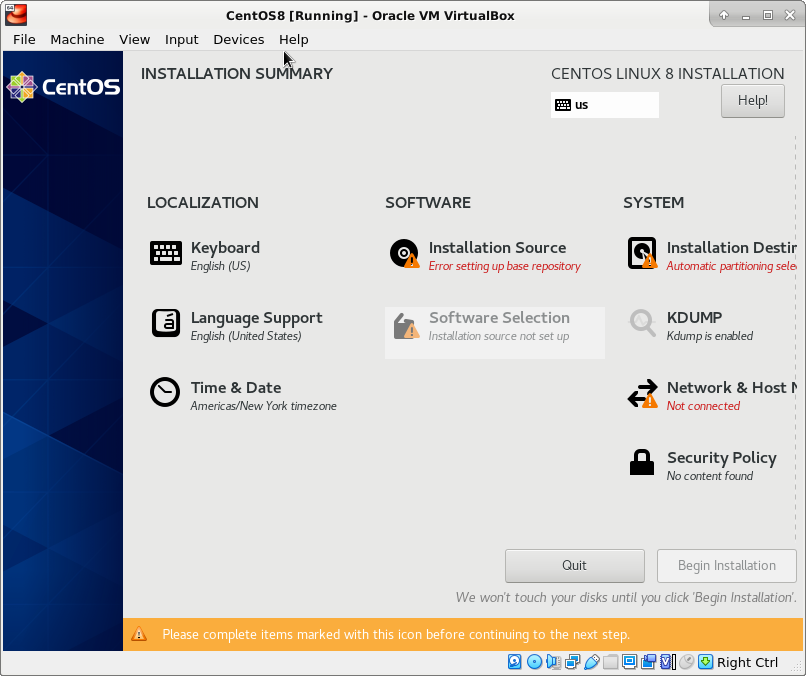
\includegraphics[width=0.99\linewidth]{linuxreader-img009.png}%
		}
		\end{minipage}
	\item We beginnen met Network \& Host Name. In het menu dat verschijnt hoef je het netwerk alleen maar op On te zetten en dan op Done te clicken.
	\item Vervolgens selecteren we Time \& Date en zetten we de tijdzone naar Europe en de plaats Amsterdam. En als dat nog niet aan staat dan zetten we Network time ook op On. Daarna clicken we weer Done.
	\item Nu gaan we voor de Installation Destination optie. Om het makkelijk te houden gaan we volledig voor de standaard instellingen, dus selecteren we Done.
	\item En als laatste kiezen we voor Installation Source. Aan de linkerkant selecteren we Workstation en aan de rechterkant zetten we een vinkje voor Office Suite and Productivity, we sluiten weer af met Done.
	\item Nu is de knop Begin Installation donker grijs geworden en kunnen we hem aanclicken.
	\item
		\begin{minipage}[t]{\linewidth}
		\raggedright
		Het systeem zal bezig gaan met de installatie en het geeft ons ondertussen de tijd om een wachtwoord voor root (Administrator van een Linux systeem) in te stellen en een gebruikersaccount voor onszelf te maken. Doe dit alle twee en zorg dat je de wachtwoorden goed onthoud of ergens opslaat.
		\adjustbox{valign=t}{%
			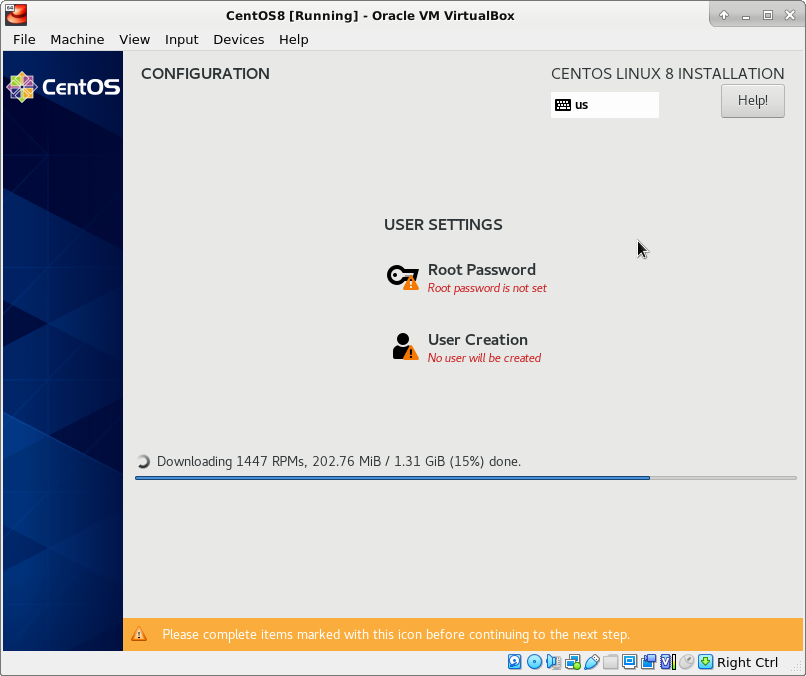
\includegraphics[width=0.99\linewidth]{linuxreader-img010.png}%
		}
		\end{minipage}
	\item Als de installatie klaar is dan moeten we via Settings $\rightarrow $ Storage de CD uit de virtuele CD speler verwijderen. Daarna kunnen we op Reboot clicken en zal ons nieuwe systeem opstarten.
	\item
		\begin{minipage}[t]{\linewidth}
		\raggedright
		\adjustbox{valign=t}{%
			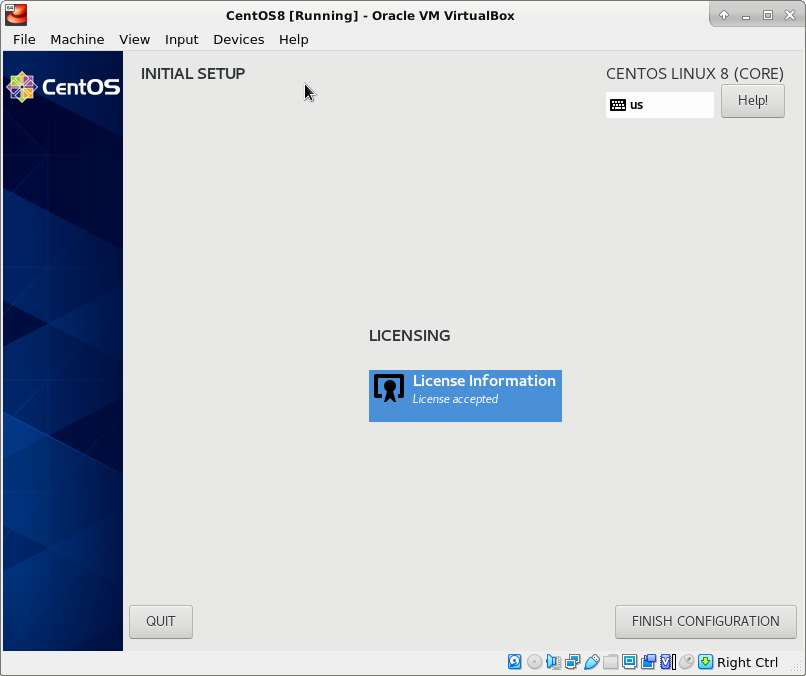
\includegraphics[width=0.99\linewidth]{linuxreader-img011.png}%
		}
		Na het opstarten en inloggen zal het systeem ons vragen om de licentievoorwaarden te accepteren.
		\end{minipage}

	\item Zodra je dit gedaan hebt kan je op FINISH CONFIGURATION clicken en zal de installatie worden afgerond.
	\item
		\begin{minipage}[t]{\linewidth}
		\raggedright
		\adjustbox{valign=t}{%
			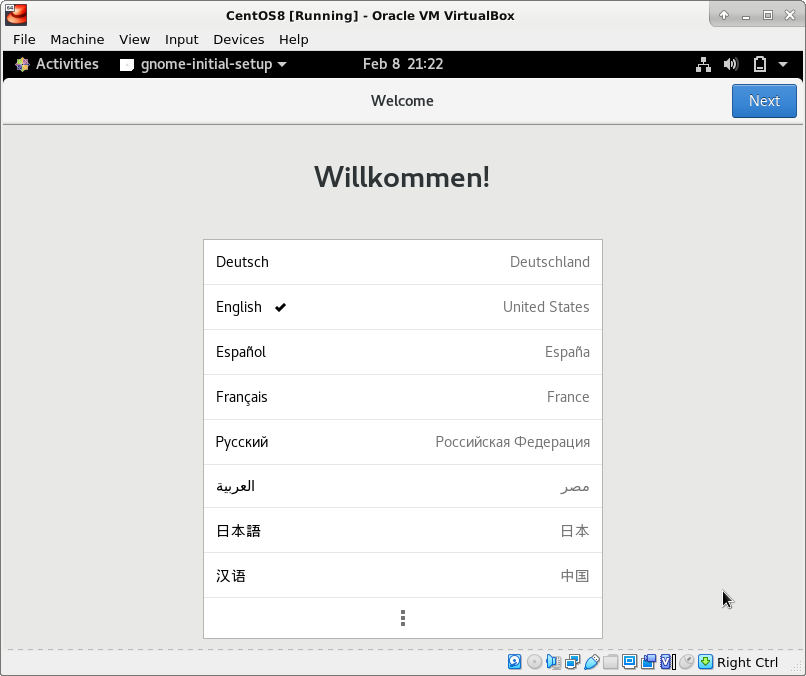
\includegraphics[width=0.99\linewidth]{linuxreader-img012.png}%
		}
		Je komt nu in het welkomstscherm terecht.
		\end{minipage}
	\item [META] Reinstall en zie wat er na Next komt en documenteer dit.
\end{enumerate}
